\documentclass[twoside]{book}

% Packages required by doxygen
\usepackage{fixltx2e}
\usepackage{calc}
\usepackage{doxygen}
\usepackage[export]{adjustbox} % also loads graphicx
\usepackage{graphicx}
\usepackage[utf8]{inputenc}
\usepackage{makeidx}
\usepackage{multicol}
\usepackage{multirow}
\PassOptionsToPackage{warn}{textcomp}
\usepackage{textcomp}
\usepackage[nointegrals]{wasysym}
\usepackage[table]{xcolor}

% Font selection
\usepackage[T1]{fontenc}
\usepackage[scaled=.90]{helvet}
\usepackage{courier}
\usepackage{amssymb}
\usepackage{sectsty}
\renewcommand{\familydefault}{\sfdefault}
\allsectionsfont{%
  \fontseries{bc}\selectfont%
  \color{darkgray}%
}
\renewcommand{\DoxyLabelFont}{%
  \fontseries{bc}\selectfont%
  \color{darkgray}%
}
\newcommand{\+}{\discretionary{\mbox{\scriptsize$\hookleftarrow$}}{}{}}

% Page & text layout
\usepackage{geometry}
\geometry{%
  a4paper,%
  top=2.5cm,%
  bottom=2.5cm,%
  left=2.5cm,%
  right=2.5cm%
}
\tolerance=750
\hfuzz=15pt
\hbadness=750
\setlength{\emergencystretch}{15pt}
\setlength{\parindent}{0cm}
\setlength{\parskip}{0.2cm}
\makeatletter
\renewcommand{\paragraph}{%
  \@startsection{paragraph}{4}{0ex}{-1.0ex}{1.0ex}{%
    \normalfont\normalsize\bfseries\SS@parafont%
  }%
}
\renewcommand{\subparagraph}{%
  \@startsection{subparagraph}{5}{0ex}{-1.0ex}{1.0ex}{%
    \normalfont\normalsize\bfseries\SS@subparafont%
  }%
}
\makeatother

% Headers & footers
\usepackage{fancyhdr}
\pagestyle{fancyplain}
\fancyhead[LE]{\fancyplain{}{\bfseries\thepage}}
\fancyhead[CE]{\fancyplain{}{}}
\fancyhead[RE]{\fancyplain{}{\bfseries\leftmark}}
\fancyhead[LO]{\fancyplain{}{\bfseries\rightmark}}
\fancyhead[CO]{\fancyplain{}{}}
\fancyhead[RO]{\fancyplain{}{\bfseries\thepage}}
\fancyfoot[LE]{\fancyplain{}{}}
\fancyfoot[CE]{\fancyplain{}{}}
\fancyfoot[RE]{\fancyplain{}{\bfseries\scriptsize Generated on Mon Sep 21 2015 23\+:18\+:33 for Aria by Doxygen }}
\fancyfoot[LO]{\fancyplain{}{\bfseries\scriptsize Generated on Mon Sep 21 2015 23\+:18\+:33 for Aria by Doxygen }}
\fancyfoot[CO]{\fancyplain{}{}}
\fancyfoot[RO]{\fancyplain{}{}}
\renewcommand{\footrulewidth}{0.4pt}
\renewcommand{\chaptermark}[1]{%
  \markboth{#1}{}%
}
\renewcommand{\sectionmark}[1]{%
  \markright{\thesection\ #1}%
}

% Indices & bibliography
\usepackage{natbib}
\usepackage[titles]{tocloft}
\setcounter{tocdepth}{3}
\setcounter{secnumdepth}{5}
\makeindex

% Hyperlinks (required, but should be loaded last)
\usepackage{ifpdf}
\ifpdf
  \usepackage[pdftex,pagebackref=true]{hyperref}
\else
  \usepackage[ps2pdf,pagebackref=true]{hyperref}
\fi
\hypersetup{%
  colorlinks=true,%
  linkcolor=blue,%
  citecolor=blue,%
  unicode%
}

% Custom commands
\newcommand{\clearemptydoublepage}{%
  \newpage{\pagestyle{empty}\cleardoublepage}%
}


%===== C O N T E N T S =====

\begin{document}

% Titlepage & ToC
\hypersetup{pageanchor=false,
             bookmarks=true,
             bookmarksnumbered=true,
             pdfencoding=unicode
            }
\pagenumbering{roman}
\begin{titlepage}
\vspace*{7cm}
\begin{center}%
{\Large Aria }\\
\vspace*{1cm}
{\large Generated by Doxygen 1.8.10}\\
\vspace*{0.5cm}
{\small Mon Sep 21 2015 23:18:33}\\
\end{center}
\end{titlepage}
\clearemptydoublepage
\tableofcontents
\clearemptydoublepage
\pagenumbering{arabic}
\hypersetup{pageanchor=true}

%--- Begin generated contents ---
\chapter{Namespace Index}
\section{Namespace List}
Here is a list of all namespaces with brief descriptions\+:\begin{DoxyCompactList}
\item\contentsline{section}{\hyperlink{namespaceAriaAttribute}{Aria\+Attribute} \\*Aria notification attribute handler }{\pageref{namespaceAriaAttribute}}{}
\item\contentsline{section}{\hyperlink{namespaceAriaMap}{Aria\+Map} \\*Aria notification shared memory handler }{\pageref{namespaceAriaMap}}{}
\item\contentsline{section}{\hyperlink{namespaceAriaUtility}{Aria\+Utility} \\*The Aria utility tool }{\pageref{namespaceAriaUtility}}{}
\end{DoxyCompactList}

\chapter{Hierarchical Index}
\section{Class Hierarchy}
This inheritance list is sorted roughly, but not completely, alphabetically\+:\begin{DoxyCompactList}
\item \contentsline{section}{Map\+Data}{\pageref{structMapData}}{}
\item Window\begin{DoxyCompactList}
\item \contentsline{section}{Aria\+Notify}{\pageref{classAriaNotify}}{}
\end{DoxyCompactList}
\end{DoxyCompactList}

\chapter{Class Index}
\section{Class List}
Here are the classes, structs, unions and interfaces with brief descriptions\+:\begin{DoxyCompactList}
\item\contentsline{section}{\hyperlink{classAriaNotify}{Aria\+Notify} \\*Aria notification bubble object }{\pageref{classAriaNotify}}{}
\item\contentsline{section}{\hyperlink{structMapData}{Map\+Data} }{\pageref{structMapData}}{}
\end{DoxyCompactList}

\chapter{File Index}
\section{File List}
Here is a list of all files with brief descriptions\+:\begin{DoxyCompactList}
\item\contentsline{section}{common/include/\hyperlink{AriaAttribute_8h}{Aria\+Attribute.\+h} }{\pageref{AriaAttribute_8h}}{}
\item\contentsline{section}{common/include/\hyperlink{AriaUtility_8h}{Aria\+Utility.\+h} }{\pageref{AriaUtility_8h}}{}
\item\contentsline{section}{common/src/\hyperlink{AriaAttribute_8cc}{Aria\+Attribute.\+cc} }{\pageref{AriaAttribute_8cc}}{}
\item\contentsline{section}{common/src/\hyperlink{AriaUtility_8cc}{Aria\+Utility.\+cc} }{\pageref{AriaUtility_8cc}}{}
\item\contentsline{section}{core/include/\hyperlink{AriaMap_8h}{Aria\+Map.\+h} }{\pageref{AriaMap_8h}}{}
\item\contentsline{section}{core/include/\hyperlink{AriaNotify_8h}{Aria\+Notify.\+h} }{\pageref{AriaNotify_8h}}{}
\item\contentsline{section}{core/src/\hyperlink{aria_8cc}{aria.\+cc} }{\pageref{aria_8cc}}{}
\item\contentsline{section}{core/src/\hyperlink{AriaMap_8cc}{Aria\+Map.\+cc} }{\pageref{AriaMap_8cc}}{}
\item\contentsline{section}{core/src/\hyperlink{AriaNotify_8cc}{Aria\+Notify.\+cc} }{\pageref{AriaNotify_8cc}}{}
\end{DoxyCompactList}

\chapter{Namespace Documentation}
\hypertarget{namespaceAriaAttribute}{}\section{Aria\+Attribute Namespace Reference}
\label{namespaceAriaAttribute}\index{Aria\+Attribute@{Aria\+Attribute}}


Aria notification attribute handler.  


\subsection*{Functions}
\begin{DoxyCompactItemize}
\item 
int \hyperlink{namespaceAriaAttribute_a3a5236d92709e7f388d3b9a1518600c8}{init} (char $\ast$$\ast$argv)
\begin{DoxyCompactList}\small\item\em Initialize the Aria attribute data structure by populating some user defined pieces. \end{DoxyCompactList}\item 
int \hyperlink{namespaceAriaAttribute_af61c3761904e3565cf2aebe81b6c47e7}{setstr} (std\+::string key, std\+::string val)
\begin{DoxyCompactList}\small\item\em Set values in the attribute data structure using a key-\/value pairing system. \end{DoxyCompactList}\item 
int \hyperlink{namespaceAriaAttribute_a2bd079b87e4ecbce0caa2935c3bfad1a}{setint} (std\+::string key, int val)
\begin{DoxyCompactList}\small\item\em Set values in the attribute data structure using a key-\/value pairing system. \end{DoxyCompactList}\item 
int \hyperlink{namespaceAriaAttribute_a6e836e2e4bf4fe7932ed03c177803ac3}{setdef} (void)
\begin{DoxyCompactList}\small\item\em Set default values in the attribute data structure by reading and parsing the configuration file. \end{DoxyCompactList}\item 
std\+::string \hyperlink{namespaceAriaAttribute_a0520d9c63a5d56d843824d19ba47468b}{getstr} (std\+::string key)
\begin{DoxyCompactList}\small\item\em Return the value in the attribute data structure that is pointed to by the given key. \end{DoxyCompactList}\item 
int \hyperlink{namespaceAriaAttribute_afb6f2f13f38521cc9ac3c9b29ab2a31d}{getint} (std\+::string key)
\begin{DoxyCompactList}\small\item\em Return the value in the attribute data structure that is pointed to by the given key. \end{DoxyCompactList}\item 
void \hyperlink{namespaceAriaAttribute_ac4e511c856781ac1fa0e1b527d9b8688}{print} (void)
\begin{DoxyCompactList}\small\item\em Print every key-\/value pair in the attribute data structure. \end{DoxyCompactList}\end{DoxyCompactItemize}


\subsection{Detailed Description}
Aria notification attribute handler. 

Stores the data structure that contains all attributes for the Aria notification bubble. Is capable of searching, accessing, and modifying elements in the attribute data structure and returning the appropriate value back to the user. 

\subsection{Function Documentation}
\hypertarget{namespaceAriaAttribute_afb6f2f13f38521cc9ac3c9b29ab2a31d}{}\index{Aria\+Attribute@{Aria\+Attribute}!getint@{getint}}
\index{getint@{getint}!Aria\+Attribute@{Aria\+Attribute}}
\subsubsection[{getint(std\+::string key)}]{\setlength{\rightskip}{0pt plus 5cm}int Aria\+Attribute\+::getint (
\begin{DoxyParamCaption}
\item[{std\+::string}]{key}
\end{DoxyParamCaption}
)}\label{namespaceAriaAttribute_afb6f2f13f38521cc9ac3c9b29ab2a31d}


Return the value in the attribute data structure that is pointed to by the given key. 

key the unique identifier in the attribute data structure which points to a value. \hypertarget{namespaceAriaAttribute_a0520d9c63a5d56d843824d19ba47468b}{}\index{Aria\+Attribute@{Aria\+Attribute}!getstr@{getstr}}
\index{getstr@{getstr}!Aria\+Attribute@{Aria\+Attribute}}
\subsubsection[{getstr(std\+::string key)}]{\setlength{\rightskip}{0pt plus 5cm}std\+::string Aria\+Attribute\+::getstr (
\begin{DoxyParamCaption}
\item[{std\+::string}]{key}
\end{DoxyParamCaption}
)}\label{namespaceAriaAttribute_a0520d9c63a5d56d843824d19ba47468b}


Return the value in the attribute data structure that is pointed to by the given key. 

key the unique identifier in the attribute data structure which points to a value. \hypertarget{namespaceAriaAttribute_a3a5236d92709e7f388d3b9a1518600c8}{}\index{Aria\+Attribute@{Aria\+Attribute}!init@{init}}
\index{init@{init}!Aria\+Attribute@{Aria\+Attribute}}
\subsubsection[{init(char $\ast$$\ast$argv)}]{\setlength{\rightskip}{0pt plus 5cm}int Aria\+Attribute\+::init (
\begin{DoxyParamCaption}
\item[{char $\ast$$\ast$}]{argv}
\end{DoxyParamCaption}
)}\label{namespaceAriaAttribute_a3a5236d92709e7f388d3b9a1518600c8}


Initialize the Aria attribute data structure by populating some user defined pieces. 

Essentially a specialized getopt. Loop through the argument vector searching for user defined pieces and populate the data structure when a new piece is found. When all user defined pieces are specified, fill in the remainder with defaults.

argv the command line argument vector. \hypertarget{namespaceAriaAttribute_ac4e511c856781ac1fa0e1b527d9b8688}{}\index{Aria\+Attribute@{Aria\+Attribute}!print@{print}}
\index{print@{print}!Aria\+Attribute@{Aria\+Attribute}}
\subsubsection[{print(void)}]{\setlength{\rightskip}{0pt plus 5cm}void Aria\+Attribute\+::print (
\begin{DoxyParamCaption}
\item[{void}]{}
\end{DoxyParamCaption}
)}\label{namespaceAriaAttribute_ac4e511c856781ac1fa0e1b527d9b8688}


Print every key-\/value pair in the attribute data structure. 

\hypertarget{namespaceAriaAttribute_a6e836e2e4bf4fe7932ed03c177803ac3}{}\index{Aria\+Attribute@{Aria\+Attribute}!setdef@{setdef}}
\index{setdef@{setdef}!Aria\+Attribute@{Aria\+Attribute}}
\subsubsection[{setdef(void)}]{\setlength{\rightskip}{0pt plus 5cm}int Aria\+Attribute\+::setdef (
\begin{DoxyParamCaption}
\item[{void}]{}
\end{DoxyParamCaption}
)}\label{namespaceAriaAttribute_a6e836e2e4bf4fe7932ed03c177803ac3}


Set default values in the attribute data structure by reading and parsing the configuration file. 

\hypertarget{namespaceAriaAttribute_a2bd079b87e4ecbce0caa2935c3bfad1a}{}\index{Aria\+Attribute@{Aria\+Attribute}!setint@{setint}}
\index{setint@{setint}!Aria\+Attribute@{Aria\+Attribute}}
\subsubsection[{setint(std\+::string key, int val)}]{\setlength{\rightskip}{0pt plus 5cm}int Aria\+Attribute\+::setint (
\begin{DoxyParamCaption}
\item[{std\+::string}]{key, }
\item[{int}]{val}
\end{DoxyParamCaption}
)}\label{namespaceAriaAttribute_a2bd079b87e4ecbce0caa2935c3bfad1a}


Set values in the attribute data structure using a key-\/value pairing system. 

key the unique identifier in the attribute data structure which points to a value.  val the value which the key points to. \hypertarget{namespaceAriaAttribute_af61c3761904e3565cf2aebe81b6c47e7}{}\index{Aria\+Attribute@{Aria\+Attribute}!setstr@{setstr}}
\index{setstr@{setstr}!Aria\+Attribute@{Aria\+Attribute}}
\subsubsection[{setstr(std\+::string key, std\+::string val)}]{\setlength{\rightskip}{0pt plus 5cm}int Aria\+Attribute\+::setstr (
\begin{DoxyParamCaption}
\item[{std\+::string}]{key, }
\item[{std\+::string}]{val}
\end{DoxyParamCaption}
)}\label{namespaceAriaAttribute_af61c3761904e3565cf2aebe81b6c47e7}


Set values in the attribute data structure using a key-\/value pairing system. 

key the unique identifier in the attribute data structure which points to a value.  val the value which the key points to. 
\hypertarget{namespaceAriaMap}{}\section{Aria\+Map Namespace Reference}
\label{namespaceAriaMap}\index{Aria\+Map@{Aria\+Map}}
\subsection*{Functions}
\begin{DoxyCompactItemize}
\item 
int \hyperlink{namespaceAriaMap_ab476269022f8048bbb7618a4830eeabd}{store} (struct \hyperlink{structMapData}{Map\+Data} $\ast$data, long shift)
\item 
int \hyperlink{namespaceAriaMap_aad25e1bc6cbd702fd569df804d90e464}{displace} (struct \hyperlink{structMapData}{Map\+Data} $\ast$data, long shift)
\item 
int \hyperlink{namespaceAriaMap_a0820778a918ad835c8b7b9dbd2b0ae9e}{cleanup} (void)
\item 
int \hyperlink{namespaceAriaMap_a7775ad4992d7a25a554896bc3ed5e4ce}{openfd} (void)
\item 
int \hyperlink{namespaceAriaMap_ae9ed69be092b57caff848ae611339adf}{writefd} (struct \hyperlink{structMapData}{Map\+Data} $\ast$w, size\+\_\+t s)
\item 
int \hyperlink{namespaceAriaMap_a85b66efeb9b3e717ea5c8ee3f72bec1a}{readfd} (struct \hyperlink{structMapData}{Map\+Data} $\ast$r, size\+\_\+t s)
\item 
int \hyperlink{namespaceAriaMap_a4f96bec0326c57c4fb11595fb5e48e52}{clearfd} (void)
\item 
int \hyperlink{namespaceAriaMap_a16dcceca67f06165428001241996ab14}{map} (void)
\item 
int \hyperlink{namespaceAriaMap_a05e8b260d9c410e0dec752d41e22dd98}{unmap} (void)
\item 
int \hyperlink{namespaceAriaMap_abde04797d8f7dca3a40b492d7e7788a6}{insert} (struct \hyperlink{structMapData}{Map\+Data} $\ast$data)
\item 
int \hyperlink{namespaceAriaMap_af2742e0765093c4fc620caaaa76c38bc}{copy} (bool status)
\item 
int \hyperlink{namespaceAriaMap_a9d3f96512f5841571994008631b27b48}{find} (long val)
\item 
void \hyperlink{namespaceAriaMap_a1ae3654679044db830871fa3b0d409f1}{clear} (void)
\item 
void \hyperlink{namespaceAriaMap_a16bcb7ece1c6912d7372d15f38b8057e}{clear} (long start, long len)
\item 
size\+\_\+t \hyperlink{namespaceAriaMap_a6e02547a1c5f23b8b520faaf4ac435d5}{size} (void)
\item 
size\+\_\+t \hyperlink{namespaceAriaMap_a234dc58cf6e47d321f7a9743fd2635ec}{length} (void)
\item 
void \hyperlink{namespaceAriaMap_a2c1667afce41963288cba56437c48df2}{print} (void)
\end{DoxyCompactItemize}


\subsection{Function Documentation}
\hypertarget{namespaceAriaMap_a0820778a918ad835c8b7b9dbd2b0ae9e}{}\index{Aria\+Map@{Aria\+Map}!cleanup@{cleanup}}
\index{cleanup@{cleanup}!Aria\+Map@{Aria\+Map}}
\subsubsection[{cleanup(void)}]{\setlength{\rightskip}{0pt plus 5cm}int Aria\+Map\+::cleanup (
\begin{DoxyParamCaption}
\item[{void}]{}
\end{DoxyParamCaption}
)}\label{namespaceAriaMap_a0820778a918ad835c8b7b9dbd2b0ae9e}
\hypertarget{namespaceAriaMap_a1ae3654679044db830871fa3b0d409f1}{}\index{Aria\+Map@{Aria\+Map}!clear@{clear}}
\index{clear@{clear}!Aria\+Map@{Aria\+Map}}
\subsubsection[{clear(void)}]{\setlength{\rightskip}{0pt plus 5cm}void Aria\+Map\+::clear (
\begin{DoxyParamCaption}
\item[{void}]{}
\end{DoxyParamCaption}
)}\label{namespaceAriaMap_a1ae3654679044db830871fa3b0d409f1}
\hypertarget{namespaceAriaMap_a16bcb7ece1c6912d7372d15f38b8057e}{}\index{Aria\+Map@{Aria\+Map}!clear@{clear}}
\index{clear@{clear}!Aria\+Map@{Aria\+Map}}
\subsubsection[{clear(long start, long len)}]{\setlength{\rightskip}{0pt plus 5cm}void Aria\+Map\+::clear (
\begin{DoxyParamCaption}
\item[{long}]{start, }
\item[{long}]{len}
\end{DoxyParamCaption}
)}\label{namespaceAriaMap_a16bcb7ece1c6912d7372d15f38b8057e}
\hypertarget{namespaceAriaMap_a4f96bec0326c57c4fb11595fb5e48e52}{}\index{Aria\+Map@{Aria\+Map}!clearfd@{clearfd}}
\index{clearfd@{clearfd}!Aria\+Map@{Aria\+Map}}
\subsubsection[{clearfd(void)}]{\setlength{\rightskip}{0pt plus 5cm}int Aria\+Map\+::clearfd (
\begin{DoxyParamCaption}
\item[{void}]{}
\end{DoxyParamCaption}
)}\label{namespaceAriaMap_a4f96bec0326c57c4fb11595fb5e48e52}
\hypertarget{namespaceAriaMap_af2742e0765093c4fc620caaaa76c38bc}{}\index{Aria\+Map@{Aria\+Map}!copy@{copy}}
\index{copy@{copy}!Aria\+Map@{Aria\+Map}}
\subsubsection[{copy(bool status)}]{\setlength{\rightskip}{0pt plus 5cm}int Aria\+Map\+::copy (
\begin{DoxyParamCaption}
\item[{bool}]{status}
\end{DoxyParamCaption}
)}\label{namespaceAriaMap_af2742e0765093c4fc620caaaa76c38bc}
\hypertarget{namespaceAriaMap_aad25e1bc6cbd702fd569df804d90e464}{}\index{Aria\+Map@{Aria\+Map}!displace@{displace}}
\index{displace@{displace}!Aria\+Map@{Aria\+Map}}
\subsubsection[{displace(struct Map\+Data $\ast$data, long shift)}]{\setlength{\rightskip}{0pt plus 5cm}int Aria\+Map\+::displace (
\begin{DoxyParamCaption}
\item[{struct {\bf Map\+Data} $\ast$}]{data, }
\item[{long}]{shift}
\end{DoxyParamCaption}
)}\label{namespaceAriaMap_aad25e1bc6cbd702fd569df804d90e464}
\hypertarget{namespaceAriaMap_a9d3f96512f5841571994008631b27b48}{}\index{Aria\+Map@{Aria\+Map}!find@{find}}
\index{find@{find}!Aria\+Map@{Aria\+Map}}
\subsubsection[{find(long val)}]{\setlength{\rightskip}{0pt plus 5cm}int Aria\+Map\+::find (
\begin{DoxyParamCaption}
\item[{long}]{val}
\end{DoxyParamCaption}
)}\label{namespaceAriaMap_a9d3f96512f5841571994008631b27b48}
\hypertarget{namespaceAriaMap_abde04797d8f7dca3a40b492d7e7788a6}{}\index{Aria\+Map@{Aria\+Map}!insert@{insert}}
\index{insert@{insert}!Aria\+Map@{Aria\+Map}}
\subsubsection[{insert(struct Map\+Data $\ast$data)}]{\setlength{\rightskip}{0pt plus 5cm}int Aria\+Map\+::insert (
\begin{DoxyParamCaption}
\item[{struct {\bf Map\+Data} $\ast$}]{data}
\end{DoxyParamCaption}
)}\label{namespaceAriaMap_abde04797d8f7dca3a40b492d7e7788a6}
\hypertarget{namespaceAriaMap_a234dc58cf6e47d321f7a9743fd2635ec}{}\index{Aria\+Map@{Aria\+Map}!length@{length}}
\index{length@{length}!Aria\+Map@{Aria\+Map}}
\subsubsection[{length(void)}]{\setlength{\rightskip}{0pt plus 5cm}size\+\_\+t Aria\+Map\+::length (
\begin{DoxyParamCaption}
\item[{void}]{}
\end{DoxyParamCaption}
)}\label{namespaceAriaMap_a234dc58cf6e47d321f7a9743fd2635ec}
\hypertarget{namespaceAriaMap_a16dcceca67f06165428001241996ab14}{}\index{Aria\+Map@{Aria\+Map}!map@{map}}
\index{map@{map}!Aria\+Map@{Aria\+Map}}
\subsubsection[{map(void)}]{\setlength{\rightskip}{0pt plus 5cm}int Aria\+Map\+::map (
\begin{DoxyParamCaption}
\item[{void}]{}
\end{DoxyParamCaption}
)}\label{namespaceAriaMap_a16dcceca67f06165428001241996ab14}
\hypertarget{namespaceAriaMap_a7775ad4992d7a25a554896bc3ed5e4ce}{}\index{Aria\+Map@{Aria\+Map}!openfd@{openfd}}
\index{openfd@{openfd}!Aria\+Map@{Aria\+Map}}
\subsubsection[{openfd(void)}]{\setlength{\rightskip}{0pt plus 5cm}int Aria\+Map\+::openfd (
\begin{DoxyParamCaption}
\item[{void}]{}
\end{DoxyParamCaption}
)}\label{namespaceAriaMap_a7775ad4992d7a25a554896bc3ed5e4ce}
\hypertarget{namespaceAriaMap_a2c1667afce41963288cba56437c48df2}{}\index{Aria\+Map@{Aria\+Map}!print@{print}}
\index{print@{print}!Aria\+Map@{Aria\+Map}}
\subsubsection[{print(void)}]{\setlength{\rightskip}{0pt plus 5cm}void Aria\+Map\+::print (
\begin{DoxyParamCaption}
\item[{void}]{}
\end{DoxyParamCaption}
)}\label{namespaceAriaMap_a2c1667afce41963288cba56437c48df2}
\hypertarget{namespaceAriaMap_a85b66efeb9b3e717ea5c8ee3f72bec1a}{}\index{Aria\+Map@{Aria\+Map}!readfd@{readfd}}
\index{readfd@{readfd}!Aria\+Map@{Aria\+Map}}
\subsubsection[{readfd(struct Map\+Data $\ast$r, size\+\_\+t s)}]{\setlength{\rightskip}{0pt plus 5cm}int Aria\+Map\+::readfd (
\begin{DoxyParamCaption}
\item[{struct {\bf Map\+Data} $\ast$}]{r, }
\item[{size\+\_\+t}]{s}
\end{DoxyParamCaption}
)}\label{namespaceAriaMap_a85b66efeb9b3e717ea5c8ee3f72bec1a}
\hypertarget{namespaceAriaMap_a6e02547a1c5f23b8b520faaf4ac435d5}{}\index{Aria\+Map@{Aria\+Map}!size@{size}}
\index{size@{size}!Aria\+Map@{Aria\+Map}}
\subsubsection[{size(void)}]{\setlength{\rightskip}{0pt plus 5cm}size\+\_\+t Aria\+Map\+::size (
\begin{DoxyParamCaption}
\item[{void}]{}
\end{DoxyParamCaption}
)}\label{namespaceAriaMap_a6e02547a1c5f23b8b520faaf4ac435d5}
\hypertarget{namespaceAriaMap_ab476269022f8048bbb7618a4830eeabd}{}\index{Aria\+Map@{Aria\+Map}!store@{store}}
\index{store@{store}!Aria\+Map@{Aria\+Map}}
\subsubsection[{store(struct Map\+Data $\ast$data, long shift)}]{\setlength{\rightskip}{0pt plus 5cm}int Aria\+Map\+::store (
\begin{DoxyParamCaption}
\item[{struct {\bf Map\+Data} $\ast$}]{data, }
\item[{long}]{shift}
\end{DoxyParamCaption}
)}\label{namespaceAriaMap_ab476269022f8048bbb7618a4830eeabd}
\hypertarget{namespaceAriaMap_a05e8b260d9c410e0dec752d41e22dd98}{}\index{Aria\+Map@{Aria\+Map}!unmap@{unmap}}
\index{unmap@{unmap}!Aria\+Map@{Aria\+Map}}
\subsubsection[{unmap(void)}]{\setlength{\rightskip}{0pt plus 5cm}int Aria\+Map\+::unmap (
\begin{DoxyParamCaption}
\item[{void}]{}
\end{DoxyParamCaption}
)}\label{namespaceAriaMap_a05e8b260d9c410e0dec752d41e22dd98}
\hypertarget{namespaceAriaMap_ae9ed69be092b57caff848ae611339adf}{}\index{Aria\+Map@{Aria\+Map}!writefd@{writefd}}
\index{writefd@{writefd}!Aria\+Map@{Aria\+Map}}
\subsubsection[{writefd(struct Map\+Data $\ast$w, size\+\_\+t s)}]{\setlength{\rightskip}{0pt plus 5cm}int Aria\+Map\+::writefd (
\begin{DoxyParamCaption}
\item[{struct {\bf Map\+Data} $\ast$}]{w, }
\item[{size\+\_\+t}]{s}
\end{DoxyParamCaption}
)}\label{namespaceAriaMap_ae9ed69be092b57caff848ae611339adf}

\hypertarget{namespaceAriaUtility}{}\section{Aria\+Utility Namespace Reference}
\label{namespaceAriaUtility}\index{Aria\+Utility@{Aria\+Utility}}


The Aria utility tool.  


\subsection*{Functions}
\begin{DoxyCompactItemize}
\item 
void \hyperlink{namespaceAriaUtility_ab7e1ed799d49b08e2213e48cf66d441a}{usage} (void)
\item 
void \hyperlink{namespaceAriaUtility_a6f2e8e4929437544f4164fb7df5d4c11}{error} (std\+::string str)
\end{DoxyCompactItemize}


\subsection{Detailed Description}
The Aria utility tool. 

Mainly used for printing usage and error state checking. 

\subsection{Function Documentation}
\hypertarget{namespaceAriaUtility_a6f2e8e4929437544f4164fb7df5d4c11}{}\index{Aria\+Utility@{Aria\+Utility}!error@{error}}
\index{error@{error}!Aria\+Utility@{Aria\+Utility}}
\subsubsection[{error(std\+::string str)}]{\setlength{\rightskip}{0pt plus 5cm}void Aria\+Utility\+::error (
\begin{DoxyParamCaption}
\item[{std\+::string}]{str}
\end{DoxyParamCaption}
)}\label{namespaceAriaUtility_a6f2e8e4929437544f4164fb7df5d4c11}
\hypertarget{namespaceAriaUtility_ab7e1ed799d49b08e2213e48cf66d441a}{}\index{Aria\+Utility@{Aria\+Utility}!usage@{usage}}
\index{usage@{usage}!Aria\+Utility@{Aria\+Utility}}
\subsubsection[{usage(void)}]{\setlength{\rightskip}{0pt plus 5cm}void Aria\+Utility\+::usage (
\begin{DoxyParamCaption}
\item[{void}]{}
\end{DoxyParamCaption}
)}\label{namespaceAriaUtility_ab7e1ed799d49b08e2213e48cf66d441a}

\chapter{Class Documentation}
\hypertarget{classAriaNotify}{}\section{Aria\+Notify Class Reference}
\label{classAriaNotify}\index{Aria\+Notify@{Aria\+Notify}}


Aria notification bubble object.  




{\ttfamily \#include $<$Aria\+Notify.\+h$>$}

Inheritance diagram for Aria\+Notify\+:\begin{figure}[H]
\begin{center}
\leavevmode
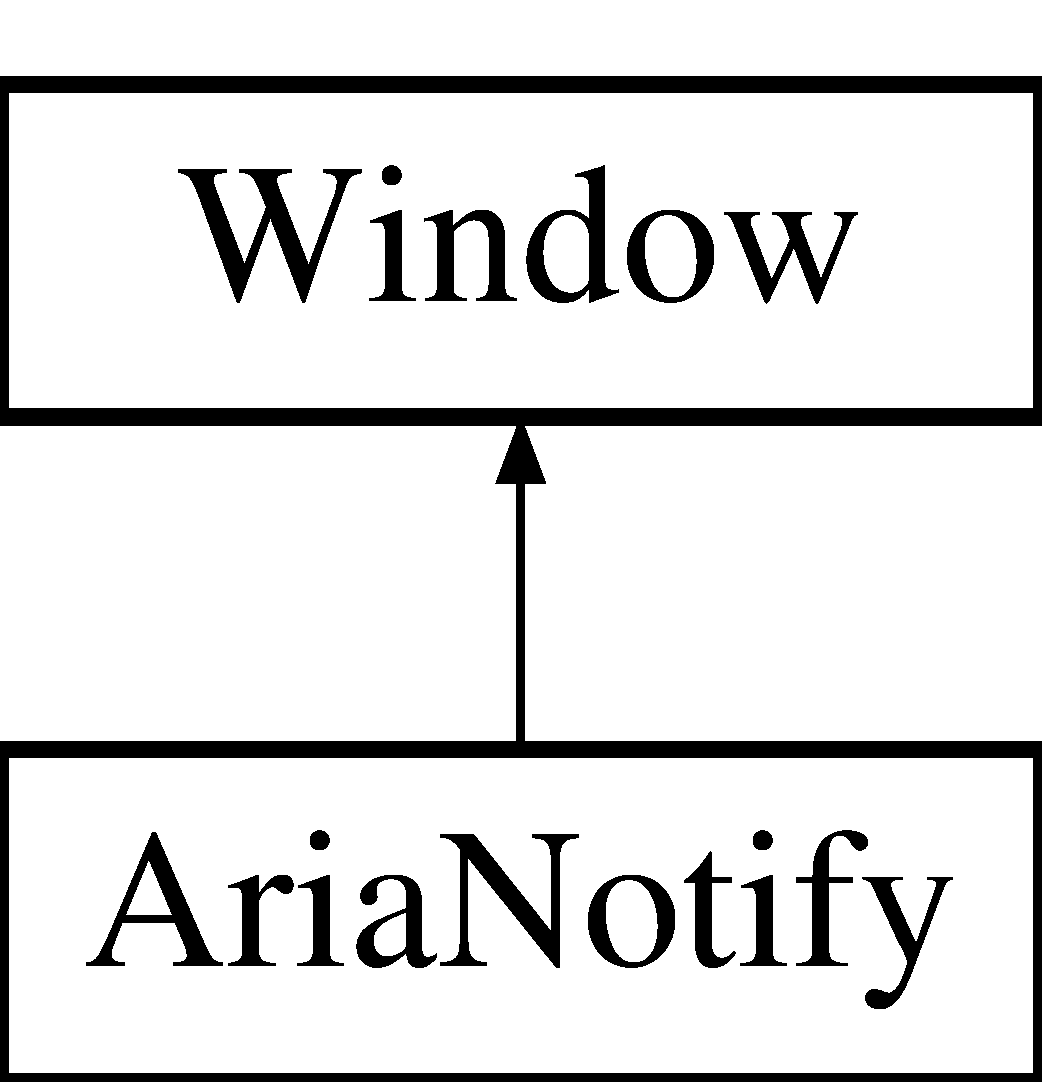
\includegraphics[height=2.000000cm]{classAriaNotify}
\end{center}
\end{figure}
\subsection*{Public Member Functions}
\begin{DoxyCompactItemize}
\item 
\hyperlink{classAriaNotify_a12a3c30e76a779224eda9b85ab64da41}{Aria\+Notify} ()
\item 
void \hyperlink{classAriaNotify_a44b553e65a193d1d6def4158bbdbb2ae}{init} (char $\ast$$\ast$argv)
\begin{DoxyCompactList}\small\item\em Initialize the notification bubble. \end{DoxyCompactList}\item 
void \hyperlink{classAriaNotify_a36bb378b4e4f3cfaa3415674c40e5ddb}{show} (void)
\begin{DoxyCompactList}\small\item\em Display the notification bubble. \end{DoxyCompactList}\item 
void \hyperlink{classAriaNotify_a67f8b8c529ac7066b533e7de1dead607}{position} (void)
\begin{DoxyCompactList}\small\item\em Move the notification bubble. \end{DoxyCompactList}\item 
void \hyperlink{classAriaNotify_ab6c049c98062b55fb9dbf93ad86506be}{set\+\_\+title} (void)
\begin{DoxyCompactList}\small\item\em Set the notification bubble title text. \end{DoxyCompactList}\item 
void \hyperlink{classAriaNotify_aad084fc44a4896dbd096fc94da77d911}{set\+\_\+body} (void)
\begin{DoxyCompactList}\small\item\em Set the notification bubble body text. \end{DoxyCompactList}\item 
void \hyperlink{classAriaNotify_ad733a27ee37e049400d91814d6cec659}{set\+\_\+notify\+\_\+text} (std\+::string field)
\begin{DoxyCompactList}\small\item\em General notification text setter. \end{DoxyCompactList}\item 
void \hyperlink{classAriaNotify_a3070b81ec7549551985807608c4dc230}{set\+\_\+background} (void)
\begin{DoxyCompactList}\small\item\em Set the background color of the notification bubble. \end{DoxyCompactList}\item 
void \hyperlink{classAriaNotify_a8befc6cd8cc6c3bfd9fb498ca43149df}{set\+\_\+foreground} (void)
\begin{DoxyCompactList}\small\item\em Set the foreground (text) color of the notification bubble. \end{DoxyCompactList}\item 
void \hyperlink{classAriaNotify_abdc3c582bed37b641270135f701f8c94}{set\+\_\+margin} (void)
\begin{DoxyCompactList}\small\item\em Set the margin of the notification bubble text. \end{DoxyCompactList}\item 
void \hyperlink{classAriaNotify_ac3a070a586a3ac7470479c23bb8619c1}{set\+\_\+size} (void)
\begin{DoxyCompactList}\small\item\em Set the notification bubble size. \end{DoxyCompactList}\item 
void \hyperlink{classAriaNotify_a11a1357c1243a781dabcce8c545838e4}{set\+\_\+timer} (void)
\begin{DoxyCompactList}\small\item\em Set the notification bubble timer. \end{DoxyCompactList}\end{DoxyCompactItemize}
\subsection*{Static Public Member Functions}
\begin{DoxyCompactItemize}
\item 
static void \hyperlink{classAriaNotify_ae9a1c13596ad8a7b1f363755c43ee72a}{cleanup} (int sig)
\begin{DoxyCompactList}\small\item\em Cleanup any memory mapped data. \end{DoxyCompactList}\end{DoxyCompactItemize}
\subsection*{Public Attributes}
\begin{DoxyCompactItemize}
\item 
Gtk\+::\+Box \hyperlink{classAriaNotify_acf839bd737ad1f569e868a886f1760f5}{bubble}
\end{DoxyCompactItemize}


\subsection{Detailed Description}
Aria notification bubble object. 

Handles the initialization, creation, and displaying of the notification bubble. 

\subsection{Constructor \& Destructor Documentation}
\hypertarget{classAriaNotify_a12a3c30e76a779224eda9b85ab64da41}{}\index{Aria\+Notify@{Aria\+Notify}!Aria\+Notify@{Aria\+Notify}}
\index{Aria\+Notify@{Aria\+Notify}!Aria\+Notify@{Aria\+Notify}}
\subsubsection[{Aria\+Notify()}]{\setlength{\rightskip}{0pt plus 5cm}Aria\+Notify\+::\+Aria\+Notify (
\begin{DoxyParamCaption}
{}
\end{DoxyParamCaption}
)}\label{classAriaNotify_a12a3c30e76a779224eda9b85ab64da41}
Construct the notification window and container. 

\subsection{Member Function Documentation}
\hypertarget{classAriaNotify_ae9a1c13596ad8a7b1f363755c43ee72a}{}\index{Aria\+Notify@{Aria\+Notify}!cleanup@{cleanup}}
\index{cleanup@{cleanup}!Aria\+Notify@{Aria\+Notify}}
\subsubsection[{cleanup(int sig)}]{\setlength{\rightskip}{0pt plus 5cm}void Aria\+Notify\+::cleanup (
\begin{DoxyParamCaption}
\item[{int}]{sig}
\end{DoxyParamCaption}
)\hspace{0.3cm}{\ttfamily [static]}}\label{classAriaNotify_ae9a1c13596ad8a7b1f363755c43ee72a}


Cleanup any memory mapped data. 

Shuts down the program after cleaning up stored data. Used as a static member function due to its status as a signal handler.


\begin{DoxyParams}{Parameters}
{\em sig} & the signal that was raised. Incidentally, also the exit status. \\
\hline
\end{DoxyParams}
\hypertarget{classAriaNotify_a44b553e65a193d1d6def4158bbdbb2ae}{}\index{Aria\+Notify@{Aria\+Notify}!init@{init}}
\index{init@{init}!Aria\+Notify@{Aria\+Notify}}
\subsubsection[{init(char $\ast$$\ast$argv)}]{\setlength{\rightskip}{0pt plus 5cm}void Aria\+Notify\+::init (
\begin{DoxyParamCaption}
\item[{char $\ast$$\ast$}]{argv}
\end{DoxyParamCaption}
)}\label{classAriaNotify_a44b553e65a193d1d6def4158bbdbb2ae}


Initialize the notification bubble. 

Check inputs and set up signal handlers for cleanup.


\begin{DoxyParams}{Parameters}
{\em argv} & the command line argument vector. \\
\hline
\end{DoxyParams}
\hypertarget{classAriaNotify_a67f8b8c529ac7066b533e7de1dead607}{}\index{Aria\+Notify@{Aria\+Notify}!position@{position}}
\index{position@{position}!Aria\+Notify@{Aria\+Notify}}
\subsubsection[{position(void)}]{\setlength{\rightskip}{0pt plus 5cm}void Aria\+Notify\+::position (
\begin{DoxyParamCaption}
\item[{void}]{}
\end{DoxyParamCaption}
)}\label{classAriaNotify_a67f8b8c529ac7066b533e7de1dead607}


Move the notification bubble. 

Determine the appropriate location to move the notification bubble such that there will be no overlap with other notifications. Stores this position in a shared memory region as a means of interprocess communication with other Aria applications. \hypertarget{classAriaNotify_a3070b81ec7549551985807608c4dc230}{}\index{Aria\+Notify@{Aria\+Notify}!set\+\_\+background@{set\+\_\+background}}
\index{set\+\_\+background@{set\+\_\+background}!Aria\+Notify@{Aria\+Notify}}
\subsubsection[{set\+\_\+background(void)}]{\setlength{\rightskip}{0pt plus 5cm}void Aria\+Notify\+::set\+\_\+background (
\begin{DoxyParamCaption}
\item[{void}]{}
\end{DoxyParamCaption}
)}\label{classAriaNotify_a3070b81ec7549551985807608c4dc230}


Set the background color of the notification bubble. 

\hypertarget{classAriaNotify_aad084fc44a4896dbd096fc94da77d911}{}\index{Aria\+Notify@{Aria\+Notify}!set\+\_\+body@{set\+\_\+body}}
\index{set\+\_\+body@{set\+\_\+body}!Aria\+Notify@{Aria\+Notify}}
\subsubsection[{set\+\_\+body(void)}]{\setlength{\rightskip}{0pt plus 5cm}void Aria\+Notify\+::set\+\_\+body (
\begin{DoxyParamCaption}
\item[{void}]{}
\end{DoxyParamCaption}
)}\label{classAriaNotify_aad084fc44a4896dbd096fc94da77d911}


Set the notification bubble body text. 

\hypertarget{classAriaNotify_a8befc6cd8cc6c3bfd9fb498ca43149df}{}\index{Aria\+Notify@{Aria\+Notify}!set\+\_\+foreground@{set\+\_\+foreground}}
\index{set\+\_\+foreground@{set\+\_\+foreground}!Aria\+Notify@{Aria\+Notify}}
\subsubsection[{set\+\_\+foreground(void)}]{\setlength{\rightskip}{0pt plus 5cm}void Aria\+Notify\+::set\+\_\+foreground (
\begin{DoxyParamCaption}
\item[{void}]{}
\end{DoxyParamCaption}
)}\label{classAriaNotify_a8befc6cd8cc6c3bfd9fb498ca43149df}


Set the foreground (text) color of the notification bubble. 

\hypertarget{classAriaNotify_abdc3c582bed37b641270135f701f8c94}{}\index{Aria\+Notify@{Aria\+Notify}!set\+\_\+margin@{set\+\_\+margin}}
\index{set\+\_\+margin@{set\+\_\+margin}!Aria\+Notify@{Aria\+Notify}}
\subsubsection[{set\+\_\+margin(void)}]{\setlength{\rightskip}{0pt plus 5cm}void Aria\+Notify\+::set\+\_\+margin (
\begin{DoxyParamCaption}
\item[{void}]{}
\end{DoxyParamCaption}
)}\label{classAriaNotify_abdc3c582bed37b641270135f701f8c94}


Set the margin of the notification bubble text. 

\hypertarget{classAriaNotify_ad733a27ee37e049400d91814d6cec659}{}\index{Aria\+Notify@{Aria\+Notify}!set\+\_\+notify\+\_\+text@{set\+\_\+notify\+\_\+text}}
\index{set\+\_\+notify\+\_\+text@{set\+\_\+notify\+\_\+text}!Aria\+Notify@{Aria\+Notify}}
\subsubsection[{set\+\_\+notify\+\_\+text(std\+::string field)}]{\setlength{\rightskip}{0pt plus 5cm}void Aria\+Notify\+::set\+\_\+notify\+\_\+text (
\begin{DoxyParamCaption}
\item[{std\+::string}]{field}
\end{DoxyParamCaption}
)}\label{classAriaNotify_ad733a27ee37e049400d91814d6cec659}


General notification text setter. 

Set the font family, font size, and text for the given notification field.


\begin{DoxyParams}{Parameters}
{\em field} & the notification field to setup -\/ either title or body. \\
\hline
\end{DoxyParams}
\hypertarget{classAriaNotify_ac3a070a586a3ac7470479c23bb8619c1}{}\index{Aria\+Notify@{Aria\+Notify}!set\+\_\+size@{set\+\_\+size}}
\index{set\+\_\+size@{set\+\_\+size}!Aria\+Notify@{Aria\+Notify}}
\subsubsection[{set\+\_\+size(void)}]{\setlength{\rightskip}{0pt plus 5cm}void Aria\+Notify\+::set\+\_\+size (
\begin{DoxyParamCaption}
\item[{void}]{}
\end{DoxyParamCaption}
)}\label{classAriaNotify_ac3a070a586a3ac7470479c23bb8619c1}


Set the notification bubble size. 

\hypertarget{classAriaNotify_a11a1357c1243a781dabcce8c545838e4}{}\index{Aria\+Notify@{Aria\+Notify}!set\+\_\+timer@{set\+\_\+timer}}
\index{set\+\_\+timer@{set\+\_\+timer}!Aria\+Notify@{Aria\+Notify}}
\subsubsection[{set\+\_\+timer(void)}]{\setlength{\rightskip}{0pt plus 5cm}void Aria\+Notify\+::set\+\_\+timer (
\begin{DoxyParamCaption}
\item[{void}]{}
\end{DoxyParamCaption}
)}\label{classAriaNotify_a11a1357c1243a781dabcce8c545838e4}


Set the notification bubble timer. 

Closes the notification bubble after the timeout. \hypertarget{classAriaNotify_ab6c049c98062b55fb9dbf93ad86506be}{}\index{Aria\+Notify@{Aria\+Notify}!set\+\_\+title@{set\+\_\+title}}
\index{set\+\_\+title@{set\+\_\+title}!Aria\+Notify@{Aria\+Notify}}
\subsubsection[{set\+\_\+title(void)}]{\setlength{\rightskip}{0pt plus 5cm}void Aria\+Notify\+::set\+\_\+title (
\begin{DoxyParamCaption}
\item[{void}]{}
\end{DoxyParamCaption}
)}\label{classAriaNotify_ab6c049c98062b55fb9dbf93ad86506be}


Set the notification bubble title text. 

\hypertarget{classAriaNotify_a36bb378b4e4f3cfaa3415674c40e5ddb}{}\index{Aria\+Notify@{Aria\+Notify}!show@{show}}
\index{show@{show}!Aria\+Notify@{Aria\+Notify}}
\subsubsection[{show(void)}]{\setlength{\rightskip}{0pt plus 5cm}void Aria\+Notify\+::show (
\begin{DoxyParamCaption}
\item[{void}]{}
\end{DoxyParamCaption}
)}\label{classAriaNotify_a36bb378b4e4f3cfaa3415674c40e5ddb}


Display the notification bubble. 



\subsection{Member Data Documentation}
\hypertarget{classAriaNotify_acf839bd737ad1f569e868a886f1760f5}{}\index{Aria\+Notify@{Aria\+Notify}!bubble@{bubble}}
\index{bubble@{bubble}!Aria\+Notify@{Aria\+Notify}}
\subsubsection[{bubble}]{\setlength{\rightskip}{0pt plus 5cm}Gtk\+::\+Box Aria\+Notify\+::bubble}\label{classAriaNotify_acf839bd737ad1f569e868a886f1760f5}


The documentation for this class was generated from the following files\+:\begin{DoxyCompactItemize}
\item 
core/include/\hyperlink{AriaNotify_8h}{Aria\+Notify.\+h}\item 
core/src/\hyperlink{AriaNotify_8cc}{Aria\+Notify.\+cc}\end{DoxyCompactItemize}

\hypertarget{structMapData}{}\section{Map\+Data Struct Reference}
\label{structMapData}\index{Map\+Data@{Map\+Data}}


{\ttfamily \#include $<$Aria\+Map.\+h$>$}

\subsection*{Public Attributes}
\begin{DoxyCompactItemize}
\item 
long \hyperlink{structMapData_ad27eaf83bb30b0b46e224d5cd78b34b7}{id}
\item 
long \hyperlink{structMapData_a52a37fc0f0cb1564824d68a86d0d4c97}{x}
\item 
long \hyperlink{structMapData_ace819161d4cd3db76cac2f104a9fb78d}{y}
\item 
long \hyperlink{structMapData_a7cc187013c2f397ddbb575ac065fe25e}{w}
\item 
long \hyperlink{structMapData_a31903efa4d79958802ee06a0f268b24a}{h}
\end{DoxyCompactItemize}


\subsection{Member Data Documentation}
\hypertarget{structMapData_a31903efa4d79958802ee06a0f268b24a}{}\index{Map\+Data@{Map\+Data}!h@{h}}
\index{h@{h}!Map\+Data@{Map\+Data}}
\subsubsection[{h}]{\setlength{\rightskip}{0pt plus 5cm}long Map\+Data\+::h}\label{structMapData_a31903efa4d79958802ee06a0f268b24a}
\hypertarget{structMapData_ad27eaf83bb30b0b46e224d5cd78b34b7}{}\index{Map\+Data@{Map\+Data}!id@{id}}
\index{id@{id}!Map\+Data@{Map\+Data}}
\subsubsection[{id}]{\setlength{\rightskip}{0pt plus 5cm}long Map\+Data\+::id}\label{structMapData_ad27eaf83bb30b0b46e224d5cd78b34b7}
\hypertarget{structMapData_a7cc187013c2f397ddbb575ac065fe25e}{}\index{Map\+Data@{Map\+Data}!w@{w}}
\index{w@{w}!Map\+Data@{Map\+Data}}
\subsubsection[{w}]{\setlength{\rightskip}{0pt plus 5cm}long Map\+Data\+::w}\label{structMapData_a7cc187013c2f397ddbb575ac065fe25e}
\hypertarget{structMapData_a52a37fc0f0cb1564824d68a86d0d4c97}{}\index{Map\+Data@{Map\+Data}!x@{x}}
\index{x@{x}!Map\+Data@{Map\+Data}}
\subsubsection[{x}]{\setlength{\rightskip}{0pt plus 5cm}long Map\+Data\+::x}\label{structMapData_a52a37fc0f0cb1564824d68a86d0d4c97}
\hypertarget{structMapData_ace819161d4cd3db76cac2f104a9fb78d}{}\index{Map\+Data@{Map\+Data}!y@{y}}
\index{y@{y}!Map\+Data@{Map\+Data}}
\subsubsection[{y}]{\setlength{\rightskip}{0pt plus 5cm}long Map\+Data\+::y}\label{structMapData_ace819161d4cd3db76cac2f104a9fb78d}


The documentation for this struct was generated from the following file\+:\begin{DoxyCompactItemize}
\item 
core/include/\hyperlink{AriaMap_8h}{Aria\+Map.\+h}\end{DoxyCompactItemize}

\chapter{File Documentation}
\hypertarget{AriaAttribute_8h}{}\section{common/include/\+Aria\+Attribute.h File Reference}
\label{AriaAttribute_8h}\index{common/include/\+Aria\+Attribute.\+h@{common/include/\+Aria\+Attribute.\+h}}
{\ttfamily \#include $<$string$>$}\\*
\subsection*{Namespaces}
\begin{DoxyCompactItemize}
\item 
 \hyperlink{namespaceAriaAttribute}{Aria\+Attribute}
\begin{DoxyCompactList}\small\item\em Aria notification attribute handler. \end{DoxyCompactList}\end{DoxyCompactItemize}
\subsection*{Functions}
\begin{DoxyCompactItemize}
\item 
int \hyperlink{namespaceAriaAttribute_a3a5236d92709e7f388d3b9a1518600c8}{Aria\+Attribute\+::init} (char $\ast$$\ast$argv)
\begin{DoxyCompactList}\small\item\em Initialize the Aria attribute data structure by populating some user defined pieces. \end{DoxyCompactList}\item 
int \hyperlink{namespaceAriaAttribute_af61c3761904e3565cf2aebe81b6c47e7}{Aria\+Attribute\+::setstr} (std\+::string key, std\+::string val)
\begin{DoxyCompactList}\small\item\em Set values in the attribute data structure using a key-\/value pairing system. \end{DoxyCompactList}\item 
int \hyperlink{namespaceAriaAttribute_a2bd079b87e4ecbce0caa2935c3bfad1a}{Aria\+Attribute\+::setint} (std\+::string key, int val)
\begin{DoxyCompactList}\small\item\em Set values in the attribute data structure using a key-\/value pairing system. \end{DoxyCompactList}\item 
int \hyperlink{namespaceAriaAttribute_a6e836e2e4bf4fe7932ed03c177803ac3}{Aria\+Attribute\+::setdef} (void)
\begin{DoxyCompactList}\small\item\em Set default values in the attribute data structure by reading and parsing the configuration file. \end{DoxyCompactList}\item 
std\+::string \hyperlink{namespaceAriaAttribute_a0520d9c63a5d56d843824d19ba47468b}{Aria\+Attribute\+::getstr} (std\+::string key)
\begin{DoxyCompactList}\small\item\em Return the value in the attribute data structure that is pointed to by the given key. \end{DoxyCompactList}\item 
int \hyperlink{namespaceAriaAttribute_afb6f2f13f38521cc9ac3c9b29ab2a31d}{Aria\+Attribute\+::getint} (std\+::string key)
\begin{DoxyCompactList}\small\item\em Return the value in the attribute data structure that is pointed to by the given key. \end{DoxyCompactList}\item 
void \hyperlink{namespaceAriaAttribute_ac4e511c856781ac1fa0e1b527d9b8688}{Aria\+Attribute\+::print} (void)
\begin{DoxyCompactList}\small\item\em Print every key-\/value pair in the attribute data structure. \end{DoxyCompactList}\end{DoxyCompactItemize}

\hypertarget{AriaUtility_8h}{}\section{common/include/\+Aria\+Utility.h File Reference}
\label{AriaUtility_8h}\index{common/include/\+Aria\+Utility.\+h@{common/include/\+Aria\+Utility.\+h}}
{\ttfamily \#include $<$string$>$}\\*
\subsection*{Namespaces}
\begin{DoxyCompactItemize}
\item 
 \hyperlink{namespaceAriaUtility}{Aria\+Utility}
\begin{DoxyCompactList}\small\item\em The Aria utility tool. \end{DoxyCompactList}\end{DoxyCompactItemize}
\subsection*{Functions}
\begin{DoxyCompactItemize}
\item 
void \hyperlink{namespaceAriaUtility_ab7e1ed799d49b08e2213e48cf66d441a}{Aria\+Utility\+::usage} (void)
\begin{DoxyCompactList}\small\item\em Print program usage. \end{DoxyCompactList}\item 
void \hyperlink{namespaceAriaUtility_a6f2e8e4929437544f4164fb7df5d4c11}{Aria\+Utility\+::error} (std\+::string str)
\begin{DoxyCompactList}\small\item\em Print error message and exit. \end{DoxyCompactList}\item 
void \hyperlink{namespaceAriaUtility_a6b433fae13ebf1b45db31c0173cd943a}{Aria\+Utility\+::checkery} (int ret, const char $\ast$str, int err)
\begin{DoxyCompactList}\small\item\em Check for errors based on the return status. \end{DoxyCompactList}\item 
void \hyperlink{namespaceAriaUtility_a22b217c239a92579332108e0f6310029}{Aria\+Utility\+::checkery} (void $\ast$ptr, const char $\ast$str, int err)
\begin{DoxyCompactList}\small\item\em Check for errors based on the return status. \end{DoxyCompactList}\end{DoxyCompactItemize}

\hypertarget{AriaAttribute_8cc}{}\section{common/src/\+Aria\+Attribute.cc File Reference}
\label{AriaAttribute_8cc}\index{common/src/\+Aria\+Attribute.\+cc@{common/src/\+Aria\+Attribute.\+cc}}
{\ttfamily \#include \char`\"{}Aria\+Attribute.\+h\char`\"{}}\\*
{\ttfamily \#include $<$X11/\+Xlib.\+h$>$}\\*
{\ttfamily \#include $<$iostream$>$}\\*
{\ttfamily \#include $<$algorithm$>$}\\*
{\ttfamily \#include $<$cctype$>$}\\*
{\ttfamily \#include $<$fstream$>$}\\*
{\ttfamily \#include $<$sstream$>$}\\*
{\ttfamily \#include $<$string$>$}\\*
\subsection*{Macros}
\begin{DoxyCompactItemize}
\item 
\#define \hyperlink{AriaAttribute_8cc_a3c7c6a69f690fc8d2abf0e385280a532}{A\+R\+R\+A\+Y\+\_\+\+S\+I\+Z\+E}(arr)~(sizeof(arr) / sizeof(arr\mbox{[}0\mbox{]}))
\end{DoxyCompactItemize}
\subsection*{Variables}
\begin{DoxyCompactItemize}
\item 
const std\+::string \hyperlink{AriaAttribute_8cc_adadc98d612a8482de299079125b660da}{C\+O\+N\+F\+\_\+\+F\+I\+L\+E} = \char`\"{}/home/gabeg/scripts/programs/aria/aria.\+conf\char`\"{}
\end{DoxyCompactItemize}


\subsection{Macro Definition Documentation}
\hypertarget{AriaAttribute_8cc_a3c7c6a69f690fc8d2abf0e385280a532}{}\index{Aria\+Attribute.\+cc@{Aria\+Attribute.\+cc}!A\+R\+R\+A\+Y\+\_\+\+S\+I\+Z\+E@{A\+R\+R\+A\+Y\+\_\+\+S\+I\+Z\+E}}
\index{A\+R\+R\+A\+Y\+\_\+\+S\+I\+Z\+E@{A\+R\+R\+A\+Y\+\_\+\+S\+I\+Z\+E}!Aria\+Attribute.\+cc@{Aria\+Attribute.\+cc}}
\subsubsection[{A\+R\+R\+A\+Y\+\_\+\+S\+I\+Z\+E}]{\setlength{\rightskip}{0pt plus 5cm}\#define A\+R\+R\+A\+Y\+\_\+\+S\+I\+Z\+E(
\begin{DoxyParamCaption}
\item[{}]{arr}
\end{DoxyParamCaption}
)~(sizeof(arr) / sizeof(arr\mbox{[}0\mbox{]}))}\label{AriaAttribute_8cc_a3c7c6a69f690fc8d2abf0e385280a532}


\subsection{Variable Documentation}
\hypertarget{AriaAttribute_8cc_adadc98d612a8482de299079125b660da}{}\index{Aria\+Attribute.\+cc@{Aria\+Attribute.\+cc}!C\+O\+N\+F\+\_\+\+F\+I\+L\+E@{C\+O\+N\+F\+\_\+\+F\+I\+L\+E}}
\index{C\+O\+N\+F\+\_\+\+F\+I\+L\+E@{C\+O\+N\+F\+\_\+\+F\+I\+L\+E}!Aria\+Attribute.\+cc@{Aria\+Attribute.\+cc}}
\subsubsection[{C\+O\+N\+F\+\_\+\+F\+I\+L\+E}]{\setlength{\rightskip}{0pt plus 5cm}const std\+::string C\+O\+N\+F\+\_\+\+F\+I\+L\+E = \char`\"{}/home/gabeg/scripts/programs/aria/aria.\+conf\char`\"{}}\label{AriaAttribute_8cc_adadc98d612a8482de299079125b660da}

\hypertarget{AriaUtility_8cc}{}\section{common/src/\+Aria\+Utility.cc File Reference}
\label{AriaUtility_8cc}\index{common/src/\+Aria\+Utility.\+cc@{common/src/\+Aria\+Utility.\+cc}}
{\ttfamily \#include \char`\"{}Aria\+Utility.\+h\char`\"{}}\\*
{\ttfamily \#include \char`\"{}Aria\+Attribute.\+h\char`\"{}}\\*
{\ttfamily \#include $<$cstdlib$>$}\\*
{\ttfamily \#include $<$iostream$>$}\\*
{\ttfamily \#include $<$string$>$}\\*

\hypertarget{AriaMap_8h}{}\section{core/include/\+Aria\+Map.h File Reference}
\label{AriaMap_8h}\index{core/include/\+Aria\+Map.\+h@{core/include/\+Aria\+Map.\+h}}
{\ttfamily \#include $<$cstddef$>$}\\*
\subsection*{Classes}
\begin{DoxyCompactItemize}
\item 
struct \hyperlink{structMapData}{Map\+Data}
\end{DoxyCompactItemize}
\subsection*{Namespaces}
\begin{DoxyCompactItemize}
\item 
 \hyperlink{namespaceAriaMap}{Aria\+Map}
\end{DoxyCompactItemize}
\subsection*{Functions}
\begin{DoxyCompactItemize}
\item 
int \hyperlink{namespaceAriaMap_ab476269022f8048bbb7618a4830eeabd}{Aria\+Map\+::store} (struct \hyperlink{structMapData}{Map\+Data} $\ast$data, long shift)
\item 
int \hyperlink{namespaceAriaMap_aad25e1bc6cbd702fd569df804d90e464}{Aria\+Map\+::displace} (struct \hyperlink{structMapData}{Map\+Data} $\ast$data, long shift)
\item 
int \hyperlink{namespaceAriaMap_a0820778a918ad835c8b7b9dbd2b0ae9e}{Aria\+Map\+::cleanup} (void)
\item 
int \hyperlink{namespaceAriaMap_a7775ad4992d7a25a554896bc3ed5e4ce}{Aria\+Map\+::openfd} (void)
\item 
int \hyperlink{namespaceAriaMap_ae9ed69be092b57caff848ae611339adf}{Aria\+Map\+::writefd} (struct \hyperlink{structMapData}{Map\+Data} $\ast$w, size\+\_\+t s)
\item 
int \hyperlink{namespaceAriaMap_a85b66efeb9b3e717ea5c8ee3f72bec1a}{Aria\+Map\+::readfd} (struct \hyperlink{structMapData}{Map\+Data} $\ast$r, size\+\_\+t s)
\item 
int \hyperlink{namespaceAriaMap_a4f96bec0326c57c4fb11595fb5e48e52}{Aria\+Map\+::clearfd} (void)
\item 
int \hyperlink{namespaceAriaMap_a16dcceca67f06165428001241996ab14}{Aria\+Map\+::map} (void)
\item 
int \hyperlink{namespaceAriaMap_a05e8b260d9c410e0dec752d41e22dd98}{Aria\+Map\+::unmap} (void)
\item 
int \hyperlink{namespaceAriaMap_abde04797d8f7dca3a40b492d7e7788a6}{Aria\+Map\+::insert} (struct \hyperlink{structMapData}{Map\+Data} $\ast$data)
\item 
int \hyperlink{namespaceAriaMap_af2742e0765093c4fc620caaaa76c38bc}{Aria\+Map\+::copy} (bool status)
\item 
int \hyperlink{namespaceAriaMap_a9d3f96512f5841571994008631b27b48}{Aria\+Map\+::find} (long val)
\item 
void \hyperlink{namespaceAriaMap_a1ae3654679044db830871fa3b0d409f1}{Aria\+Map\+::clear} (void)
\item 
void \hyperlink{namespaceAriaMap_a16bcb7ece1c6912d7372d15f38b8057e}{Aria\+Map\+::clear} (long start, long len)
\item 
size\+\_\+t \hyperlink{namespaceAriaMap_a6e02547a1c5f23b8b520faaf4ac435d5}{Aria\+Map\+::size} (void)
\item 
size\+\_\+t \hyperlink{namespaceAriaMap_a234dc58cf6e47d321f7a9743fd2635ec}{Aria\+Map\+::length} (void)
\item 
void \hyperlink{namespaceAriaMap_a2c1667afce41963288cba56437c48df2}{Aria\+Map\+::print} (void)
\end{DoxyCompactItemize}

\hypertarget{AriaNotify_8h}{}\section{core/include/\+Aria\+Notify.h File Reference}
\label{AriaNotify_8h}\index{core/include/\+Aria\+Notify.\+h@{core/include/\+Aria\+Notify.\+h}}
{\ttfamily \#include $<$gtkmm.\+h$>$}\\*
{\ttfamily \#include $<$string$>$}\\*
\subsection*{Classes}
\begin{DoxyCompactItemize}
\item 
class \hyperlink{classAriaNotify}{Aria\+Notify}
\begin{DoxyCompactList}\small\item\em Aria notification bubble object. \end{DoxyCompactList}\end{DoxyCompactItemize}

\hypertarget{aria_8cc}{}\section{core/src/aria.cc File Reference}
\label{aria_8cc}\index{core/src/aria.\+cc@{core/src/aria.\+cc}}
{\ttfamily \#include \char`\"{}Aria\+Notify.\+h\char`\"{}}\\*
{\ttfamily \#include $<$gtkmm.\+h$>$}\\*
\subsection*{Functions}
\begin{DoxyCompactItemize}
\item 
int \hyperlink{aria_8cc_a3c04138a5bfe5d72780bb7e82a18e627}{main} (int argc, char $\ast$$\ast$argv)
\end{DoxyCompactItemize}


\subsection{Function Documentation}
\hypertarget{aria_8cc_a3c04138a5bfe5d72780bb7e82a18e627}{}\index{aria.\+cc@{aria.\+cc}!main@{main}}
\index{main@{main}!aria.\+cc@{aria.\+cc}}
\subsubsection[{main(int argc, char $\ast$$\ast$argv)}]{\setlength{\rightskip}{0pt plus 5cm}int main (
\begin{DoxyParamCaption}
\item[{int}]{argc, }
\item[{char $\ast$$\ast$}]{argv}
\end{DoxyParamCaption}
)}\label{aria_8cc_a3c04138a5bfe5d72780bb7e82a18e627}

\hypertarget{AriaMap_8cc}{}\section{core/src/\+Aria\+Map.cc File Reference}
\label{AriaMap_8cc}\index{core/src/\+Aria\+Map.\+cc@{core/src/\+Aria\+Map.\+cc}}
{\ttfamily \#include \char`\"{}Aria\+Map.\+h\char`\"{}}\\*
{\ttfamily \#include \char`\"{}Aria\+Utility.\+h\char`\"{}}\\*
{\ttfamily \#include $<$stdint.\+h$>$}\\*
{\ttfamily \#include $<$fcntl.\+h$>$}\\*
{\ttfamily \#include $<$unistd.\+h$>$}\\*
{\ttfamily \#include $<$sys/types.\+h$>$}\\*
{\ttfamily \#include $<$sys/stat.\+h$>$}\\*
{\ttfamily \#include $<$sys/mman.\+h$>$}\\*
{\ttfamily \#include $<$iostream$>$}\\*
{\ttfamily \#include $<$cstddef$>$}\\*
{\ttfamily \#include $<$cstdlib$>$}\\*
{\ttfamily \#include $<$cerrno$>$}\\*
{\ttfamily \#include $<$cstring$>$}\\*
{\ttfamily \#include $<$stdio.\+h$>$}\\*
{\ttfamily \#include $<$sys/file.\+h$>$}\\*

\hypertarget{AriaNotify_8cc}{}\section{core/src/\+Aria\+Notify.cc File Reference}
\label{AriaNotify_8cc}\index{core/src/\+Aria\+Notify.\+cc@{core/src/\+Aria\+Notify.\+cc}}
{\ttfamily \#include \char`\"{}Aria\+Notify.\+h\char`\"{}}\\*
{\ttfamily \#include \char`\"{}Aria\+Attribute.\+h\char`\"{}}\\*
{\ttfamily \#include \char`\"{}Aria\+Map.\+h\char`\"{}}\\*
{\ttfamily \#include \char`\"{}Aria\+Utility.\+h\char`\"{}}\\*
{\ttfamily \#include $<$gtkmm.\+h$>$}\\*
{\ttfamily \#include $<$gdkmm.\+h$>$}\\*
{\ttfamily \#include $<$pangomm/fontdescription.\+h$>$}\\*
{\ttfamily \#include $<$cstdlib$>$}\\*
{\ttfamily \#include $<$csignal$>$}\\*
{\ttfamily \#include $<$iostream$>$}\\*
{\ttfamily \#include $<$string$>$}\\*

%--- End generated contents ---

% Index
\backmatter
\newpage
\phantomsection
\clearemptydoublepage
\addcontentsline{toc}{chapter}{Index}
\printindex

\end{document}
